\documentclass[12pt, a4paper, twoside]{report} 
\usepackage{blindtext}
\usepackage{setspace}
\linespread{1.5}
\usepackage{graphicx}
\usepackage[a4paper,top=4cm,bottom=4cm,left=3cm,right=3cm,marginparwidth=1.75cm]{geometry}
\usepackage[colorlinks=true, linkcolor=blue, citecolor=red]{hyperref}
\graphicspath{{./Chapter2/}}
\usepackage{acronym}
\usepackage{amsmath}
\usepackage{amssymb}
\usepackage{fancyhdr}
\usepackage{tikz}
\usepackage{colortbl} % Required for colored table rules
\usepackage{xcolor}    % Provides color definitions
\usepackage{mathtools}
\usepackage{subcaption}
\usepackage{tikz-feynman}
\definecolor{lightgray}{rgb}{0.8,0.8,0.8} 
\usepackage{adjustbox}

\usepackage[numbers]{natbib}
%-------------
% CMS Packages
\usepackage{style/ptdr-definitions}
\usepackage{style/hepparticles}
\usepackage{style/heppennames2}
%-------------

\pagestyle{plain}  % Default plain page style
\fancypagestyle{chapterpages}{
    \fancyhf{} % Clear existing header/footer
    \fancyhead[L]{\thepage}  % Left header: Page number
    \fancyhead[R]{\nouppercase{Chapter \thechapter: \leftmark}}
    \renewcommand{\headrulewidth}{0.4pt} % Header rule
}
\renewcommand{\chaptermark}[1]{\markboth{#1}{}}


\newcommand{\hardmaths} {\frac{\sin{(x\pi)}} {2\alpha}}

\newcommand{\diff}[2]  {\frac{\textrm{d}{#1}} {\textrm{d}{#2}}}


\begin{document}


\includegraphics[width=7cm]{IMPERIAL_Wordmark_CMYK_Blue_safe_area_2024.jpg}
\vspace{5cm}
\begin{center}


{\huge Thesis Plan}
\rule{15cm}{1pt}
\vspace{2cm}

Klitos Savva\\
2025
\vspace{2cm}

Department of Physics

Imperial College London
\vspace{2cm}

Submitted in part fulfilment of the requirements for the degree of\\
Doctor of Typessetting of Imperial College London\\
and the Diploma of Imperial College London
\vfill
\clearpage
\end{center}

\chapter*{Abstract}
\blindtext

\chapter*{Statement of Originality}
\blindtext

\chapter*{Copyright Statement}
\blindtext





\tableofcontents
\listoffigures
\listoftables

%\chapter{The Standard Model of particle physics}

The \ac{SM} of particle physics is our current best theoretical framework underpinning our understanding of the subatomic world, providing a description of fundamental elementary particles and their interactions via the electromagnetic force, weak nuclear force and the strong nuclear force. The fourth fundamental force of nature, Gravity, is absent from the SM, highlighting one of its key limitations. However, in high-energy physics experiments, where the interactions of subatomic particles are being studied, the omission of gravity is considered a safe simplification. Extremely powerful predictions have emerged from this theoretical framework, with its greatest success being the discovery of the Higgs boson by the ATLAS and CMS Collaborations in 2012, completing the observational confirmation of all hypothesized SM particles. Despite its success, the Standard Model has its limitations. Along with the absence of gravity, it leaves several fundamental questions unanswered, such as the nature of neutrino oscillations, the existence of dark matter, the hierarchy problem, and the matter-antimatter asymmetry in the universe, which cannot be fully explained by the predicted amount of CP violation, driving the field to look for explanations beyond the SM. In the pursue of \ac{BSM} physics, a deep understanding of the SM theory is crucial. This is the goal of this chapter aiming to establish the base foundation for this work, the SM, taking a trip down the fundamental blocks of the theory, including its particle content, interactions, and the Higgs mechanism.

\section{Particle content}

\begin{figure}
\centering
\includegraphics[width= 1\textwidth]{Figures/Introduction/Particles.pdf}
\end{figure}

\section{Fundamental forces}
\section{Higgs mechanism}
\section{The Higgs boson}

\cite{Rowling_1997}
\cite{Thor_2011}
\chapter*{Introduction }
\addcontentsline{toc}{chapter}{Introduction}

\chapter{The Standard Model of particle physics}

The \ac{SM} of particle physics is our current best theoretical framework underpinning our understanding of the subatomic world, providing a description of fundamental elementary particles and their interactions via the electromagnetic force, weak nuclear force and the strong nuclear force. The fourth fundamental force of nature, Gravity, is absent from the SM, highlighting one of its key limitations. However, in high-energy physics experiments, where the interactions of subatomic particles are being studied, the omission of gravity is considered a safe simplification. Extremely powerful predictions have emerged from this theoretical framework, with its greatest success being the discovery of the Higgs boson by the ATLAS and CMS Collaborations in 2012, completing the observational confirmation of all hypothesized SM particles. Despite its success, the Standard Model has its limitations. Along with the absence of gravity, it leaves several fundamental questions unanswered, such as the nature of neutrino oscillations, the existence of dark matter, the hierarchy problem, and the matter-antimatter asymmetry in the universe, which cannot be fully explained by the predicted amount of CP violation, driving the field to look for explanations beyond the SM. In the pursue of \ac{BSM} physics, a deep understanding of the SM theory is crucial. This is the goal of this chapter aiming to establish the base foundation for this work, the SM, taking a trip down the fundamental blocks of the theory, including its particle content, interactions, and the Higgs mechanism.

\section{Particle content}

\begin{figure}
\centering
\includegraphics[width= 1\textwidth]{Figures/Introduction/Particles.pdf}
\end{figure}

\section{Fundamental forces}
\section{Higgs mechanism}
\section{The Higgs boson}

\cite{Rowling_1997}
\cite{Thor_2011}
\chapter{Motivation for Higgs Sector Extensions and Higgs CP Studies}
\chaptermark{Motivation for Higgs Sector Extensions and Higgs CP Studies}  
\thispagestyle{plain}  % First page has default style
\pagestyle{chapterpages}
\label{Section:Chapter2}

In Chapter~\ref{Section:Chapter1}, the SM of particle physics was explored to establish the theoretical foundation of this work. While the SM has been immensely successful, with its predictions verified experimentally to a high degree of precision, it remains an incomplete theory of nature due to several fundamental theoretical problems. Beyond these theoretical issues, the emergence of experimental results in tension with SM predictions has sparked significant interest. Although the statistical significance of these tensions is not yet sufficient to claim new discoveries, the search for BSM physics to explain them remains an intriguing and active area of research. This chapter will focus on two major theoretical challenges; the hierarchy problem and the observed matter-antimatter asymmetry of the universe, while also discussing key experimental tensions. Possible solutions within the context of BSM physics will then be explored, with the observed Higgs boson playing an integral role in the matter-antimatter asymmetry discussion.

\section{Hierarchy problem}

A fundamental principle in theoretical physics is naturalness, which suggests that parameters in a theory should not take values that are unnaturally small or large without an underlying reason. In the case of the Standard Model (SM), this concept is particularly relevant to the Higgs boson mass, which is significantly smaller than the Planck scale ($m_P \approx 10^{19} \GeV$), where gravitational interactions become as strong as other fundamental forces.

Since the SM is widely regarded as an effective field theory (EFT), valid up to a certain energy scale, it is expected to require an extension at higher energies. The hierarchy problem arises from the absence of a natural mechanism to prevent large quantum corrections from driving the Higgs boson mass to much higher scales, typically near the Planck mass. This extreme disparity between the electroweak scale ($10^2 \GeV$) and the Planck scale remains one of the most significant unresolved questions in high-energy physics.

In QFT, the Higgs boson mass in not simply a fixed parameter. It receives corrections to its physical mass from virtual processes involving particles that couple directly or indirectly to the Higgs field. Mathematically the physical mass of the Higgs boson can be expressed as

\begin{equation}
    m_H^2 = (m_H^0)^2 + \Delta m_H^2
\label{Equation:Chapter2_HiggsBosonMass}
\end{equation}

where $m_H^0$ represents the bare mass of the Higgs boson, and $\Delta m_H$ term encapsulates the quantum loop corrections. In the EFT framework, the loop-induced correction term takes the form,

\begin{equation}
    \Delta m_H^2 = -\frac{g_f^2}{8\pi^2}\Lambda^2 + \space \text{...}
\end{equation}

where $\Lambda$ should be interpreted as the least energy scale at which new physics is expected to modify the high-energy behaviour of the theory~\cite{SUSY}. The Feynman diagram for the mass correction due to a fermion coupling to the Higgs field is shown in Fig.~\ref{Figure:Chapter2_Hierarchy_Feynman1}.

\begin{figure}[h]
\centering
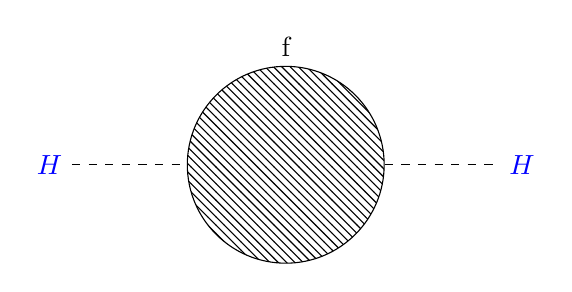
\begin{tikzpicture}
    \begin{feynman}
      \vertex[blob, minimum size=2.5cm] (m) at ( 0, 0) {};
      \vertex[blue] (a) at (-3,0){\(H\)};
      \vertex[blue] (b) at ( 3,0){\(H\)};
      \node[black] at (0,1.5) {f}; 


      \diagram* {
        (a) -- [scalar] (m) -- [scalar] (b),
      };
    \end{feynman}
\end{tikzpicture}

\caption{One-loop Feynman diagram illustrating the correction to the Higgs boson mass due to its coupling to a fermion.}
\label{Figure:Chapter2_Hierarchy_Feynman1}
\end{figure}

At the core of the hierarchy problem lies this $\Lambda$ term. If $\Lambda$ is taken to be close to the Plank scale, these quantum loop correction become many orders of magnitude larger than the observed mass of the Higgs boson, $125.04 \pm 0.12~\GeV$ (in natural units)~\cite{Higgs_Mass_Z4L}. To reconcile this, an extreme degree of fine-tuning in Eq.~\ref{Equation:Chapter2_HiggsBosonMass} is required. Specifically, the bare mass term has to be sufficiently large ($\mathcal{O}(10^{38})$) to cancel out the quantum loop correction term. This degree of unnatural finetuning remains an open question in the field, as the Higgs mass would otherwise be expected close to the scale of new physics. This could suggest that new physics may exist near $\Lambda$, that can stabilise the Higgs mass and resolve the hierarchy problem. 

Perhaps, the most studied and appealing solution to the hierarchy problem is \ac{SUSY}~\cite{SUSY}, which introduces a symmetry relating fermions and bosons. In SUSY, every known SM particle has at least one supersymmetric partner. Bosons have fermionic superpartners while, fermions have scalar boson superpartners. This symmetry provides a natural way of addressing this extreme fine-tuning, as superpartners also contribute to $\Delta m_H^2$ but, with opposite signs relative to their SM counterparts. This allows the Higgs mass to stabilise naturally through the cancellation of the quantum loop corrections. The Feynman diagram for the mass correction due to a fermionic superpartner (scalar boson) is shown in Fig.~\ref{Figure:Chapter2_Hierarchy_Feynman2}.

\begin{figure}[h]
\centering
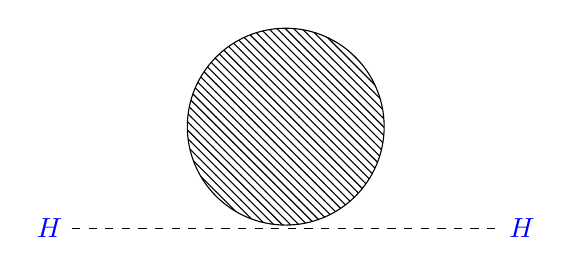
\begin{tikzpicture}
    \begin{feynman}
      \vertex[blob, minimum size=2.5cm] (m) at ( 0, 0) {};
      \vertex[blue] (a) at (-3,-1.29){\(H\)};
      \vertex[blue] (b) at ( 3,-1.29){\(H\)};

      \diagram* {
        (m),
        (a) -- [scalar] (b),
      };
    \end{feynman}
\end{tikzpicture}

\caption{One-loop correction to the Higgs mass due to a scalar S}
\label{Figure:Chapter2_Hierarchy_Feynman2}
\end{figure}

While SUSY provides a natural solution to the hierarchy problem, the lack of any experimental evidence for supersymmetric partners, along with strong experimental constraints on the simplest SUSY extension of the SM (MSSM), has lead to alternative extensions to the SM Higgs sector gaining traction. One such extension is the \ac{2HDM}, where the introduction of additional Higgs bosons that could alter the running of coupling constants and loop corrections. Moreover, 2HDMs are particularly interesting in light of the muon $g-2$ anomaly, which will be discussed in this chapter.

\section{Extended Higgs sector - 2HDM}
\label{Section:Chapter2_2HDM}
The simplest extension to the SM Higgs sector is the 2HDM~\cite{2HDM_1}. In contrast to the SM, the 2HDM introduces two complex scalar $\mathcal{SU(2)}_L$ doublets, $\Phi_1$ and $\Phi_2$.

\begin{equation}
\Phi_i =
\begin{pmatrix}
\phi_i^{+} \\
\phi_i^{0} 
\end{pmatrix}
\quad ,\quad i = 1,2
\end{equation}

The presence of the additional doublet in 2HDM leads to a richer potential structure. The general 2HDM Higgs potential, written in terms of the doublets $\Phi_1$ and $\Phi_2$, takes the form,

\begin{equation}
\begin{array}{c}
    V(\Phi_1,\Phi_2) = m_{11}^2 \Phi_1^{\dagger}\Phi_1 + m_{22}^2 \Phi_2^{\dagger}\Phi_2 - m_{12}^2(\Phi_1^\dagger\Phi_2 + \text{H.c.}) \\
    + \frac{1}{2} \lambda_1(\Phi_1^\dagger\Phi_1)^2 + \frac{1}{2}\lambda_2(\Phi_2^\dagger\Phi_2)^2 + \lambda_3(\Phi_1^\dagger\Phi_1)(\Phi_2^\dagger\Phi_2) \\
    + \lambda_4(\Phi_1^\dagger\Phi_2)(\Phi_2^\dagger\Phi_1) + \frac{1}{2}\lambda_5[(\Phi_1^\dagger\Phi_2)^2 + (\Phi_2^\dagger\Phi_1)^2] \\
    + \lambda_6(\Phi_1^\dagger\Phi_1)(\Phi_1^\dagger\Phi_2) + \lambda_7(\Phi_2^\dagger\Phi_2)(\Phi_1^\dagger\Phi_2)
\end{array}
\end{equation}

where the scalar potential is expressed in terms of the mass parameters ($m_{ij}$) and the quartic couplings ($\lambda_i$)~\cite{2HDM_1}. 

A major constraint imposed in 2HDMs is the suppression of tree-level \ac{FCNC}~\cite{FCNC_1,2HDM_2}. In a generic 2HDM, both Higgs doublets can couple to the same fermion flavour, which leads to non-diagonal Yukawa couplings after SSB. These couplings are strongly constrained by experimental data~\cite{FCNC_Constraints}. To forbid these tree-level interactions, a discrete $\mathbb{Z}_2$ symmetry \cite{2HDM_2} is introduced, 

\begin{equation}
    \Phi_1 \to \Phi_1, \Phi_2 \to - \Phi_2, \Phi_1 \not\to \Phi_2 
\end{equation}

This ensures that each fermion type couples to only one of the Higgs doublets. Following the introduction of the discrete symmetry, the quartic interaction terms $\lambda_6$ and $\lambda_7$ are eliminated from the potential. In addition to suppressing flavor-changing neutral currents (FCNCs), charge-parity (CP) symmetry plays a crucial role in ensuring the theoretical consistency of 2HDMs. CP symmetry is a fundamental symmetry in quantum field theory (QFT) that combines charge conjugation (C) and parity (P). Under a charge conjugation transformation, particles are transformed into their corresponding antiparticles whilst, parity transformations invert the spatial coordinates. In the 2HDM, CP conservation is often imposed to prevent spontaneous CP violation by requiring all free parameters in the Higgs potential to be real.

In the 2HDM, electroweak symmetry breaking occurs similarly to the SM. To preserve the $\mathcal{U}(1)_{\text{EM}}$ gauge symmetry, only the neutral components of the Higgs doublets acquire non-zero VEVs, ensuring that the photon remains massless. The vacuum structure is given by,

\begin{equation}
    <0|\Phi_i|0> = \frac{1}{\sqrt{2}} \begin{pmatrix}
        0 \\
        \nu_i
    \end{pmatrix} \quad,\quad i=1,2
\end{equation}

where $\nu_1$ and $\nu_2$ are the VEVs associated with each Higgs doublet.

After SSB, the Higgs doublets can be expanded around the minima

\begin{equation}
    \text{SSB} \rightarrow\Phi_i = \begin{pmatrix}
        \phi_i^+ \\
        \frac{1}{\sqrt{2}}(\nu_i + h_i + iz_i)
    \end{pmatrix} \quad,\quad i=1,2
\end{equation}

where the doublets have been expressed in terms of CP-even ($h_i$), CP-odd ($z_i$) and charged Higgs fields ($\phi_i^+$).

Analogous to the SM Higgs sector, the introduction of a second Higgs doublet introduces an additional four dof. Upon SSB, three out of the eight dof are absorbed as Goldstone bosons providing the $\PW^{\pm}$ and $\PZ$ bosons with longitudinal dof while the remaining five dof correspond to five physical Higgs bosons; two CP-even ($\Ph$ and $\PH$), one CP-odd (A) and two charged Higgs bosons ($\PH^{\pm}$). The mass eigenstates corresponding to these physical Higgs bosons are admixtures of the components of the two Higgs doublets,

\begin{equation}
\begin{array}{c}
     h = h_1 \sin{\alpha} - h_2 \cos{\alpha} \\
     H = - h_1 \cos{\alpha} - h_2 \sin{\alpha} \\
     H^\pm = \phi_1^+ \sin{\beta} + \phi_2^+ \cos{\beta} \\
     A = z_1 \sin{\beta} - z_2 \cos{\beta}
\end{array}
\label{Equation:Chapter2_2HDM-MassEigenstates}
\end{equation}

where the parameter $\alpha$ governs the mixing between the CP-even scalars and $\beta$ is a rotational angle that diagonalises the mass-squared matrices of the pseudoscalar and the charged Higgs. The latter is defined as,

\begin{equation}
    \tan{\beta} = \nu_2/\nu_1
\end{equation}

To ensure the theoretical consistency and predictability within the 2HDM, the degree of mixing needs to be carefully controlled. This is achieved once again through a discrete $\mathbb{Z}_2$ symmetry. However, rather being strictly imposed, the symmetry is softly broken by the $m_{12}^2$ term in the scalar potential. This soft-breaking of the symmetry allows the Yukawa couplings to remain flavour diagonal while, simultaneously allowing for mass mixing between the Higgs doublets ($\Phi_i$). CP-conserving 2HDMs are split in different types, which are defined based on which Higgs doublet couples to each fermion flavour. The four types of CP-conserving 2HDMs are shown in Table~\ref{Table:Chapter2_2HDM-Types}.

\begin{table}[h]
\centering
\renewcommand{\arraystretch}{1.5} % Increase row height
\setlength{\tabcolsep}{12pt} % Increase column width
\arrayrulecolor{black} % Ensure outer borders are black
\begin{tabular}{|c|c|c|c|c|}
\hline
    & Type I   & Type II  & Type X   & Type Y   \\ \hline \hline
$u$ & $\Phi_2$ & $\Phi_2$ & $\Phi_2$ & $\Phi_2$ \\ 
\arrayrulecolor{lightgray} \hline
$d$ & $\Phi_2$ & $\Phi_1$ & $\Phi_2$ & $\Phi_1$ \\ 
\arrayrulecolor{lightgray} \hline
$l$ & $\Phi_2$ & $\Phi_2$ & $\Phi_1$ & $\Phi_2$ \\ 
\arrayrulecolor{black} \hline
\end{tabular}
\caption{Table showing how each Higgs doublet couples to each fermion flavour in different 2HDM types.}
\label{Table:Chapter2_2HDM-Types}
\end{table}

In each 2HDM type, the structure of the Yukawa interactions depends on the specific assignment of the fermion couplings to the Higgs doublets. After SSB, the Yukawa part of the 2HDM Lagrangian can be expressed in terms of the physical Higgs mass eigenstates, up-like ($u$) and down-like($d$) quark, charged lepton ($l$) and neutrino ($\upsilon$) fields as

\begin{equation}
\begin{aligned}
    \text{SSB} \rightarrow \mathcal{L}_{Yukawa}^{2HDM} &= - \sum\limits_{f=u,d,l} \frac{m_f}{\nu} 
    \left(g_f^h \overline{f}f h + g_f^H\overline{f}f H - i g_f^A\overline{f} \gamma_5 f A \right) \\
    &\quad - \left\{ \frac{\sqrt{2}V_{ud}}{\nu} \overline{u} 
    \left(m_u g_u^A P_L + m_d g_d^A P_R \right) d H^+ \right. \\
    &\quad \left. + \frac{\sqrt{2}m_l g_{l}^A}{\nu} \overline{\upsilon
_L} l_R H^+ + H.c. \right\}
\end{aligned}
\label{Equation:Chapter2_2HDM-YukawaLagrangian}
\end{equation}

where $g_f^H,g_f^A,g_f^h$ are the normalised Yukawa couplings of the fermions to the Higgs mass eigenstates, expressed relative to the SM Higgs boson's couplings. These couplings are summarised in Table~\ref{Table:Chapter2_2HDM-Couplings} for each of the four types of 2HDMs.


\begin{table}[h]
\centering
\renewcommand{\arraystretch}{1.5} % Increase row height
\setlength{\tabcolsep}{12pt} % Increase column width
\arrayrulecolor{black} % Ensure outer borders are black
\begin{tabular}{|c|c|c|c|c|}
\hline
        & Type I                     & Type II                     & Type X                                        & Type Y                      \\ \hline \hline
$g_l^A$ & $1/\tan{\beta}$            & $\tan{\beta}$               & $\tan{\beta}$    & $-1/\tan{\beta}$            \\ \arrayrulecolor{lightgray} \hline
$g_u^A$ & $1/\tan{\beta}$            & $1/\tan{\beta}$             & $1/\tan{\beta}$                               & $1/\tan{\beta}$             \\ \arrayrulecolor{lightgray} \hline
$g_d^A$ & $1/\tan{\beta}$            & $\tan{\beta}$               & $-1/\tan{\beta}$                              & $\tan{\beta}$               \\ \arrayrulecolor{lightgray} \hline
$g_l^H$ & $\sin{\alpha}/\sin{\beta}$ & $\cos{\alpha}/\cos{\beta}$  & $\cos{\alpha}/\cos{\beta}$                    & $\sin{\alpha}/\sin{\beta}$  \\ \arrayrulecolor{lightgray} \hline
$g_u^H$ & $\sin{\alpha}/\sin{\beta}$ & $\sin{\alpha}/\sin{\beta}$  & $\sin{\alpha}/\sin{\beta}$                    & $\sin{\alpha}/\sin{\beta}$  \\ \arrayrulecolor{lightgray} \hline
$g_d^H$ & $\sin{\alpha}/\sin{\beta}$ & $\cos{\alpha}/\cos{\beta}$  & $\sin{\alpha}/\sin{\beta}$                    & $\cos{\alpha}/\cos{\beta}$  \\ \arrayrulecolor{lightgray} \hline
$g_l^h$ & $\cos{\alpha}/\sin{\beta}$ & $-\sin{\alpha}/\cos{\beta}$ & $-\sin{\alpha}/\cos{\beta}$                   & $\cos{\alpha}/\sin{\beta}$  \\ \arrayrulecolor{lightgray} \hline
$g_u^h$ & $\cos{\alpha}/\sin{\beta}$ & $\cos{\alpha}/\sin{\beta}$  & $\cos{\alpha}/\sin{\beta}$                    & $\cos{\alpha}/\sin{\beta}$  \\ \arrayrulecolor{lightgray} \hline
$g_d^h$ & $\cos{\alpha}/\sin{\beta}$ & $-\sin{\alpha}/\cos{\beta}$ & $\cos{\alpha}/\sin{\beta}$                    & $-\sin{\alpha}/\cos{\beta}$ \\ \arrayrulecolor{black} \hline
\end{tabular}
\caption{Table summarising the couplings of the different fermion groups to the neutral Higgs bosons for different 2HDM types.}
\label{Table:Chapter2_2HDM-Couplings}
\end{table}

In 2HDMs, the observed Higgs boson can be matched to the predicted CP-even bosons by a linear combination of the two mass eigenstates 

\begin{equation}
    h_{\text{obs}} = \sin{(\beta - \alpha)} h + \cos{(\beta - \alpha)} H 
\end{equation}

In the Higgs alignment limit, one of these CP-even neutral Higgs boson is the observed Higgs, which enables two possible alignment scenarios, the normal and inverted scenarios. In the normal scenario, the observed Higgs is identified as the lighter h, in contrast to H being identified as the observed Higgs in the inverted scenario. The couplings of the unmatched CP-even boson are summarised in Table~\ref{Table:Chapter2_2HDM-CouplingsAlignmentLimit} for each of the four different types of 2HDMs.

\begin{equation}
\begin{rcases}
  h_{\text{obs}} = h \\
  \cos(\beta-\alpha) = 0 
\quad \end{rcases}
\quad \text{Normal}
\label{Equation:Chapter2-NormalScenario}
\end{equation}

\begin{equation}
\begin{rcases}
  h_{\text{obs}} = H \\
  \sin(\beta-\alpha) = 0
\quad \end{rcases}
\quad \text{Inverted}
\label{Equation:Chapter2-InvertedScenario}
\end{equation}


\begin{table}[h]
\centering
\renewcommand{\arraystretch}{1.5} % Increase row height
\setlength{\tabcolsep}{12pt} % Increase column width
\arrayrulecolor{black} % Ensure outer borders are black
\begin{tabular}{|c|c|c|c|c|}
\hline
Normal (Inverted)     & Type I                     & Type II                     & Type X                                        & Type Y                      \\ \hline \hline
(-)$g_l^{H(h)}$ & $-1/\tan{\beta}$  & $\tan{\beta}$  & $\tan{\beta}$                    & $-1/\tan{\beta}$  \\ \arrayrulecolor{lightgray} \hline
(-)$g_u^{H(h)}$ & $-1/\tan{\beta}$  & $-1/\tan{\beta}$  & $-1/\tan{\beta}$                    & $-1/\tan{\beta}$  \\ \arrayrulecolor{lightgray} \hline
(-)$g_d^{H(h)}$ & $-1/\tan{\beta}$  & $\tan{\beta}$  & $-1/\tan{\beta}$                    & $\tan{\beta}$  \\ \arrayrulecolor{black} \hline
\end{tabular}
\caption{Table showing the couplings of different fermion groups to the neutral Higgs boson (not matched to the observed Higgs) for different 2HDM types. Couplings for both normal and inverted scenarios are shown in a simplified format using Eqs.~\ref{Equation:Chapter2-NormalScenario}-\ref{Equation:Chapter2-InvertedScenario}.}
\label{Table:Chapter2_2HDM-CouplingsAlignmentLimit}
\end{table}

\section{\texorpdfstring{Muon $g$-2 anomaly}{Muon g-2 anomaly}}

In 2023, Fermilab announced the most precise measurement of the anomalous magnetic moment of the muon, $\alpha_\mu$~\cite{Fermilab_g-2}. Combined with the earlier result from the Brookhaven National Laboratory, the experimental average of the muon anomaly exhibits a 5.0 standard deviations from SM prediction compiled by the Muon $g-2$ Theory Initiative in 2020~\cite{Muon_Theory_Initiative}. This is a definitely an intriguing result, as it could be a hint of BSM physics, however, caution is also warranted, as there also tensions between the different theoretical calculations that could bring the prediction closer to the experimental value.


\begin{equation}
\begin{aligned}
    \alpha_\mu (SM) &= 116591810(43) \times 10^{-11} \\
    \alpha_\mu (\text{exp}) &= 116592059(22) \times 10^{-11} \quad (0.19~\text{ppm}) \\
    \Delta \alpha_\mu &= (249\pm48) \times 10^{-11}
\end{aligned}
\end{equation}

A possible explanation for the discrepancy between the experimental measurements and the theoretical prediction of the $g-2$ anomaly can be accommodated by the 2HDM. In the 2HDM, the additional Higgs bosons can introduce loop corrections to the calculation of $\alpha_\mu$, through one-loop and two-loop Barr-Zee interactions~\cite{Barr_Zee_1,Barr_Zee_2} presented in Fig.~\ref{Figure:Chapter2_OneBarrZee} and Fig.~\ref{Figure:Chapter2_TwoBarrZee} respectively. 

\begin{figure}[h]
    \centering
    % First row
    \begin{subfigure}{0.45\textwidth}
        \centering
        \begin{tikzpicture}
    \begin{feynman}
        % Define vertices
        \vertex (L) at (0,0) {\(\mu\)};
        \vertex (R) at (6,0) {\(\mu\)};
        \vertex (M) at (3,0) [dot];
        \vertex (Photon) at (3,2) {\(\gamma\)};
        \vertex (M1) at (2,0) [dot];
        \vertex (M2) at (4,0) [dot];
        \vertex at (3,-1.15) () {\(\phi/A\)};

        % Draw diagram
        \diagram* {
            (L) -- [fermion] (M) -- [fermion] (R),
            (M) -- [photon] (Photon),
            (M1) -- [scalar, half right] (M2),
        };
    \end{feynman}
\end{tikzpicture}
    \end{subfigure}
    \hfill
    \begin{subfigure}{0.45\textwidth}
        \centering
        \raisebox{8.2mm}{\begin{tikzpicture}
    \begin{feynman}
        % Define vertices
        \vertex (L) at (0,0) {\(\mu\)};
        \vertex (a) at (2,0);
        \vertex (b) at (3,1);
        \vertex (c) at (3,2) {\(\gamma\)};
        \vertex (d) at (3,0) [dot];
        \vertex (e) at (4,0);
        \vertex (R) at (6,0) {\(\mu\)};

        \vertex at (3,-0.35) {\(\nu_\mu\)};
        \vertex at (2, 0.6) {\(H^\pm\)};
        \vertex at (4, 0.6) {\(H^\pm\)};

        % Draw diagram
        \diagram* {
            (L) -- [fermion] (a),
            (a) -- [scalar] (b),
            (b) -- [photon] (c),
            (b) -- [scalar] (e),
            (a) -- [fermion] (d) -- [fermion] (e),
            (e) -- [fermion] (R),
        };
    \end{feynman}
\end{tikzpicture}}
    \end{subfigure}

    \caption{Feynman diagrams of one-loop contributions to $\Delta\alpha_\mu$.}
    \label{Figure:Chapter2_OneBarrZee}
\end{figure}

\begin{figure}[h]
    \centering
    % First row
    \begin{subfigure}{0.45\textwidth}
        \centering
        \input{FeynmanDiagrams/TwoBarrZee_1}
    \end{subfigure}
    \hfill
    \begin{subfigure}{0.45\textwidth}
        \centering
        \begin{tikzpicture}
    \begin{feynman}
        % Define vertices
        \vertex (L) at (0,0) {\(\mu\)};
        \vertex (L1) at (2,0);
        \vertex (L2) at (4,0);
        \vertex (L3) at (6,0){\(\mu\)};

        \vertex (R1) at (2.5, 1.5);
        \vertex (R2) at (3, 2.7)[dot];
        \vertex (R3) at (3, 4){\(\gamma\)};        
        \vertex (R4) at (3.5, 1.5);

        \vertex at (1.7, 0.9){\(\phi/A\)};        
        \vertex at (4.1, 0.9){\(\gamma\)};        
        \vertex at (3.85, 2.7){\(H^\pm\)}; 

        % Draw the dashed blob (scalar-like appearance)
        \draw[thick, dashed] (3,2) circle (0.7);

        % Draw diagram
        \diagram* {
            (L) -- [fermion] (L1) -- [fermion] (L2) -- [fermion] (L3),
            (L1) -- [scalar] (R1),
            (R4) -- [photon] (L2),   
            (R2) -- [photon] (R3),
        };

        % Draw the loop with arrows
        \draw[->,line width=0.9pt] (3.7,2) -- +(0,-0.1); % Small arrow on the right side of the loop
        \draw[->,line width=0.9pt] (2.3,2) -- +(0,+0.1); % Small arrow on the left side of the loop
        \draw[->,line width=0.9pt] (3, 1.3) -- +(-0.1,0); % Small arrow on the left side of the loop

    \end{feynman}
\end{tikzpicture}
    \end{subfigure}
    
    % Add vertical space between rows
    \vspace{0.5cm}

    % Second row (centered properly)
    \begin{subfigure}{0.45\textwidth}
        \centering
        \input{FeynmanDiagrams/TwoBarrZee_3}
    \end{subfigure}

    \caption{Feynman diagrams of two-loop contributions to $\Delta\alpha_\mu$.}
    \label{Figure:Chapter2_TwoBarrZee}
\end{figure}


The one-loop contributions are mediated by $\phi$, A and H$^{\pm}$ with the contribution of $\phi$ to $\Delta\alpha_\mu$ being positive while those of A and H$^{\pm}$ are negative. The dominant contribution comes from two-loop Barr-Zee type diagrams with heavy fermions in the loop providing a positive shift to $\Delta\alpha_\mu$. The CP-odd Higgs boson contributes positively primarily through the top quark loop. However, the contribution from the additional CP-even boson can have either a positive or a negative impact, depending on $\tan{\beta}$. 

For the $g-2$ anomaly to be explained by 2HDMs, enhanced couplings between muons and the additional Higgs bosons are required. These enhanced couplings can be fascilitated by the type-II and type-X 2HDMs at large values of $\tan{\beta}$. The type-II 2HDM also features enhanced couplings to down-type quarks. This leads to gluon fusion and associated production with bottom quarks, being the dominant single Higgs boson production modes. However, finding regions of parameter space within this model that can explain the $g-2$ anomaly is challenging because of the production mechanisms being heavily constrained by experimental searches at LEP, Tevatron and LHC~\cite{TypeX_2HDM}. On the other hand, the type-X 2HDM is particularly interesting because of its hadrophobic nature, featuring suppressed up-type and down-type quark couplings with increased $\tan{\beta}$. This suppression allows it to evade the experimentally constrained quark-initiated production modes, leaving much of its parameter space relatively untouched. As a result, the type-X 2HDM remains a more viable candidate for explaining the $g-2$ anomaly. 

In addition to collider constraints, the available parameter space is further shaped by theoretical considerations including vacuum stability and perturbative unitarity, as well as electroweak precision measurements~\cite{TypeX_2HDM}. The regions where the $g-2$ anomaly can be accommodated within the type X 2HDM in both alignment scenarios are summarized in Table~\ref{Table:Chapter2_TypeX-ParameterSpace}.

\begin{table}[h]
\centering
\renewcommand{\arraystretch}{1.5} % Increase row height
\setlength{\tabcolsep}{12pt} % Increase column width
\arrayrulecolor{black} % Ensure outer borders are black
\begin{tabular}{|c|c|c|c|c|}
\hline
Alignment Scenario & $\tan{\beta}$ & $\text{m}_\phi$ {[}GeV{]} & $\text{m}_A$ {[}GeV{]} & $\text{m}_{H^\pm} {[}GeV{]}$ \\ \hline \hline
Normal             & $\geq$ 90     & 130 - 245                 & 62.5 - 145             & 95 - 285                     \\ \arrayrulecolor{lightgray} \hline
Inverted           & $\geq$ 120    & 100 - 120                 & 70 - 105               & 95 - 185 \\ \arrayrulecolor{black} \hline
\end{tabular}
\caption{Summary of the regions of parameter space can be accommodated in the context of the type-X 2HDM for both normal and inverted scenarios~\cite{TypeX_2HDM}.}
\label{Table:Chapter2_TypeX-ParameterSpace}
\end{table}

To effectively probe this region of parameter space, a non-suppressed production mode is required. The simultaneous production of two BSM Higgs bosons ($\phi$ and A) from an off-shelf Z boson is such an example. With a predicted cross-section varying between 10-300 fb (see Fig.~\ref{Figure:Chapter2_4tau_ProductionXS}) across the mass ranges outlined in Table~\ref{Table:Chapter2_TypeX-ParameterSpace}, this process is very appealing. 

\begin{figure}[h]
    \centering
    % First row
    \begin{subfigure}[b]{0.8\textwidth}
        \centering
        \includegraphics[width=\textwidth]{Figures/Chapter2/4tau_ProductionXS_NS.png}
    \end{subfigure}
    \begin{subfigure}[b]{0.8\textwidth}
        \centering
        \includegraphics[width=\textwidth]{Figures/Chapter2/4tau_ProductionXS_IS.png}
    \end{subfigure}

    \caption{Projections of the total cross-section of the $pp \to Z^* \to \phi A \to 4\tau$ process as a function of $m_\phi$ and $m_A$, presented for both alignment scenarios (NS = Normal scenario \& IS = Inverted scenario) \cite{TypeX_2HDM}.}
    \label{Figure:Chapter2_4tau_ProductionXS}
\end{figure}

At high $\tan\beta$ in the type X 2HDM, the branching fractions of BSM Higgs bosons to $\tau$ leptons are dominant, hence this process has a four $\tau$ lepton final state, as shown in Fig~\ref{Figure:Chapter2_Feynman4tau}. 

\begin{figure}[h]
\centering
\begin{tikzpicture}
    \begin{feynman}
        \vertex at (0, 2.5) (qbar) {\(\overline{q}\)};
        \vertex at (0, -2.5) (q) {\(q\)};

        \vertex at (2, 0) (Z0);
        \vertex at (4, 0) (Z1);

        \vertex at (6,1.25) (A);
        \vertex at (6,-1.25) (phi);

        \vertex at (7.9,2.5) (Atau_1){\(\tau^+\)};
        \vertex at (8, 0.5) (Atau_2){\(\tau^-\)};
        \vertex at (7.9,-2.5) (phitau_2){\(\tau^-\)};
        \vertex at (8, -0.5) (phitau_1){\(\tau^+\)};

        \vertex at (3,0.5) {\(Z^*\)};
        \vertex at (4.7,1.25) {\(A\)};
        \vertex at (4.7,-1.25) {\(\phi\)};


        \diagram*{
            (q) -- [fermion] (Z0) -- [fermion] (qbar),
            (Z0) -- [photon] (Z1),
            (Z1) -- [scalar] (A),
            (Z1) -- [scalar] (phi),

            (Atau_1) -- [fermion] (A) -- [fermion] (Atau_2),
            (phitau_1) -- [fermion] (phi) -- [fermion] (phitau_2),


        };
    \end{feynman}
\end{tikzpicture}


\caption{Feynman diagram for the production of two BSM neutral Higgs bosons from an off-shell Z boson followed by their decay to four $\tau$ leptons.}
\label{Figure:Chapter2_Feynman4tau}
\end{figure}

\section{CP Nature of the SM Higgs boson}

Despite the remarkable success of the Standard Model (SM) in describing the fundamental particles and their interactions, as discussed earlier, one of its biggest shortcomings is its inability to explain the observed matter-antimatter asymmetry in the universe~\cite{MatterAntimatter}. Several theoretical frameworks attempt to address this asymmetry, with Sakharov's model of baryogenesis being the foundation~\cite{Sakharov}. According to this model, three conditions are required to generate a baryon asymmetry:

\begin{itemize}
    \item Baryon number violation: Required to create more baryons than antibaryons. A conserved baryon number would indicate that baryons and antibaryons are created in equal amounts, leading to their annihilation.
    \item C and CP violation: Without C and CP violation, particles and antiparticles would be produced in equal amounts ($\rightarrow$ annihilation). This violation allows particles and antiparticles to exhibit different behaviours in interactions.
    \item Departure from thermal equilibrium: Required to allow the asymmetry to persist. Otherwise, any process producing a baryon asymmetry would be exactly balanced out by the reverse process.
\end{itemize}

A certain degree of CP violation is required to explain this observed baryon asymmetry. The SM provides a source of CP violation through the complex phase in the CKM matrix~\cite{CKM_1,CKM_2}. CP violation in the quark sector has been experimentally verified in various sectors~\cite{CP_QuarkSector_1, CP_QuarkSector_2, CP_QuarkSector_3, CP_QuarkSector_4, 
CP_QuarkSector_5, CP_QuarkSector_6, CP_QuarkSector_7, CP_QuarkSector_8, 
CP_QuarkSector_9, CP_QuarkSector_10, CP_QuarkSector_11, CP_QuarkSector_12, 
CP_QuarkSector_13, CP_QuarkSector_14}. However, this proves insufficient to account for the baryon asymmetry. 
Naturally, this has lead to significant interest in exploring different areas of the SM to potentially find an additional source. Simultaneously, beyond the SM framework strong indications of CP violation have also emerged in neutrino oscillations~\cite{CP_Neutrino_Oscillations}. 

The SM Higgs sector is constrained to be CP-conserving by only allowing one CP-even state to couple to other particles. If the Higgs boson exhibited a CP-odd component then, CP violation would be possible in the Higgs sector, which could potentially explain the matter-antimatter asymmetry. A type of model that includes CP-violating Higgs coupling is the 2HDM, discussed in Section~\ref{Section:Chapter2_2HDM}. The CP-conserving cases were discussed earlier but CP-violating cases also exist. In such models, the three neutral bosons (h,H,A) are not CP eigenstates, but rather admixtures of the CP-even and CP-odd components, denoted as $h_1$, $h_2$,$h_3$.

Experimentally, the CP structure of the Higgs boson can be studied by measuring the CP nature of the coupling of the Higgs boson to vector bosons and fermions. Initially, the ATLAS and CMS experiments tested several spin-parity hypotheses, excluding the pure states $0^-,1^+,1^-,2^+,2^-$ at more than 99\% confidence level via the $H\to \gamma\gamma, H\to ZZ, H\to WW$~\cite{CP_constraints_1,CP_constraints_2,CP_constraints_3} decay mechanisms. A direct comparison between pure CP-even ($0^+$) and pure CP-odd ($0^-$) hypotheses is illustrated in Fig.~\ref{Figure:Chapter2_CPevenVsCPodd}. 

\begin{figure}[h]
\centering
\includegraphics[width= 0.7\textwidth]{Figures/Chapter2/SpinParity.png}
\caption{TODO taken from Ref.~\cite{CP_constraints_2}.}
\label{Figure:Chapter2_CPevenVsCPodd}
\end{figure}

The next set of constraints came from searches for CP-odd 
HVV couplings in different Higgs production modes. The first such search was conducted in vector boson fusion (VBF) production, focusing on the 
$H\to\tau\tau$ decay channel~\cite{CP_constraints_4}. Additionally, CP-odd effects were explored in associated VH production, where the Higgs boson decays into a pair of bottom quarks ($H\to bb$)~\cite{CP_constraints_5}. Since the first set of studies into the CP structure of the Higgs, constraints on the CP-invariance were tightened for the HVV couplings and extended to Higgs Yukawa couplings to fermions \cite{CP_constraints_6,CP_constraints_7,CP_constraints_8,CP_constraints_9,CP_constraints_10,CP_constraints_11,CP_constraints_12,CP_constraints_13,CP_constraints_14,CP_constraints_15,CP_constraints_16,CP_constraints_17,CP_constraints_18,CP_constraints_19,CP_constraints_20,CP_constraints_21,CP_constraints_22}. HVV couplings are highly constrained by electroweak gauge symmetry hence, hence any CP-violating terms in such interactions must respect gauge invariance. Conversely, the Yukawa Lagrangian can be naturally modified to include a CP-odd component, allowing for CP violation.

\subsection{CP structure of the Yukawa interactions}

The SM Lagragian describing the interaction of the Higgs boson and fermions (Eq.~\ref{Equation:Introduction_YukawaLagrangian} can be generalised to include a CP-odd component,

\begin{equation}
    \text{BEH} \rightarrow \mathcal{L}_{\text{Yukawa}}^f \supset - \overline{\psi_f} (\underbrace{y_f}_{\text{CP-even}} + \underbrace{i\gamma^5\tilde{y}_f}_{\text{CP-odd}})h\psi_f
\label{Equation:Chapter2_YukawaLagrangian_CP}
\end{equation}

where $y_f$ ($\tilde{y_f}$) is the CP-even (CP-odd) Yukawa coupling constant, assumed to be of SM strength \ie $y_{SM} = \frac{g_f}{\sqrt{2}}=\frac{m_f}{\nu}\approx y_f \approx \tilde{y_f}$. Alternatively, Eq.~\ref{Equation:Chapter2_YukawaLagrangian_CP} can be rewritten in terms of the reduced Yukawa couplings (or coupling strength modifiers),

\begin{equation}
\begin{aligned}
    \kappa_f = \frac{y_f}{y_{SM}}=\frac{\nu}{m_f}y_f \\
    \tilde{\kappa_f} = \frac{\tilde{y_f}}{y_{SM}}=\frac{\nu}{m_f}\tilde{y_f} \\
\end{aligned}
\end{equation}

\begin{equation}
    \text{BEH} \rightarrow \mathcal{L}_{\text{Yukawa}}^f \supset - \frac{m_f}{\nu}\overline{\psi_f} (\underbrace{\kappa_f}_{\text{CP-even}} + \underbrace{i\gamma^5\tilde{\kappa}_f}_{\text{CP-odd}})h\psi_f
\label{Equation:Chapter2_YukawaLagrangian_CP_2}
\end{equation}

In the SM, $\kappa_f = 1$ and $\tilde{\kappa_f} = 0$, indicating a purely CP-even Higgs-fermion interaction. Conversely, a pure CP-odd coupling would be represented by $\kappa_f = 0$ and $\tilde{\kappa_f} = 1$. The interaction Lagrangian~\ref{Equation:Chapter2_YukawaLagrangian_CP_2} exhibits a linear dependency on the fermionic mass, indicating the best processes to investigate the CP structure of the interaction involve the heaviest fermions. The most interesting decays (ranked by $B_f$) involve,

\begin{itemize}
    \item $H \to b\overline{b}$: This is the process with the highest branching fraction, which is also directly related to the bottom Yukawa coupling. However, this channel offers low sensitivity because of the high QCD backgrounds and the hadronization of bottom quarks into jets, which washes out spin information, making CP-sensitive measurements challenging.

    \item $H \to \tau \tau$: This decay process can serve as a direct probe of the Yukawa CP structure since the Higgs decays \textbf{directly} to fermions. 

    \item $H \to c \overline{c}$: The sensitivity to the CP structure in this process is worse than $b\overline{b}$ because of the decreased efficiency in charm-jet tagging. Moreover, any CP violation in charm-Higgs interactions is expected to be extremely small, which is beyond the reach of current experiments.

    \item $H \to \mu \mu$: This decays process offers a clean signal with little background, because of the excellent muon reconstruction at the LHC. However, there is no established technique to measure their spin as they traverse through the particle detectors without decaying. 
\end{itemize}

\subsection{Higgs CP structure through \texorpdfstring{$H\to\tau\tau$}{H→tautau} decays}

As mentioned in the previous section, the parameters $\kappa_f$ ($\kappa_\tau$) and $\tilde{\kappa_f}$ ($\tilde{\kappa_\tau}$) represent the reduced CP-even and CP-odd couplings of the Higgs to fermions ($\tau$ leptons). These couplings can be expressed in terms of an effective mixing angle $\alpha_{\tau\tau}$ as,

\begin{equation}
\tan \alpha_{\tau\tau} = \frac{\bar{\kappa}_\tau}{\kappa_\tau} 
\begin{cases}
    \alpha_{\tau\tau} \to 0, & \text{CP-even} \\
    \alpha_{\tau\tau} \to \frac{\pi}{2}, & \text{CP-odd} \\
    \text{else}, & \text{CP-mix}
\end{cases}
\label{Equation:Chapter2-NormalScenario}
\end{equation}

In Higgs boson decays to tau leptons (\(H \to \tau^+ \tau^-\)), the spin correlations between the tau leptons provide a powerful probe of the CP nature of the Higgs coupling. These correlations manifest in the angular distributions of the tau decay products, which encode the CP properties of the interaction. The differential cross-section for the production and decay of the tau pair is given by,

\begin{equation}
\begin{array}{c}
{\displaystyle
\frac{d\sigma_{H\to\tau\tau}}{d\cos\theta^+ d\cos\theta^- d\phi^+ d\phi^-} \propto
} \\[10pt]
{\displaystyle
(1 + \cos\theta^+ \cos\theta^-) \Big(1 - c(\theta^+, \theta^-) \cos(\phi^+ - \phi^- - 2\alpha_{\tau\tau})\Big)
}
\end{array}
\label{Equation:Chapter2_TauDifferentialXS}
\end{equation}

where $c(\theta^+, \theta^-)$ is defined as $\sin(\theta^+)\sin(\theta^-)/(1+\cos(\theta^+)\cos(\theta)$. The angles $\theta^\pm$ and $\phi^\pm$ are the polar and azimuthal coordinates of the polarimetric vector (optimal estimator of the $\tau$ polarisation) taken with respect to the $\tau^\pm$ direction of flight, as illustrated in Fig~\ref{Figure:Chapter2_PolarimetricVector_Definition}.

\begin{figure}[h]
\centering
\includegraphics[width= 0.6\textwidth]{Figures/Chapter2/PolarimetricVector_Definition.png}
\caption{TODO taken from Ref.~\cite{PolarimetricVectorDefinition}.}
\label{Figure:Chapter2_PolarimetricVector_Definition}
\end{figure}

A full reconstruction of the polarimetric vector is particularly challenging in most $\tau$ decay modes because of the presence of neutrinos in the final state (see Chapter TODO). However, the angular difference ($\phi^+-\phi^-$) in Eq.~\ref{Equation:Chapter2_TauDifferentialXS} coincides with the angle between the $\tau$ lepton decay planes in the Higgs rest frame, denoted as $\phi_{CP}$. A simple illustration of the decay planes is presented in Fig.~\ref{Figure:Chapter2_DecayPlanes}.

\begin{figure}[h]
\centering
\includegraphics[width= 0.6\textwidth]{Figures/Chapter2/DecayPlanes.png}
\caption{explain this is single prong TODO taken from Ref.~\cite{HiggsCP_CMS_2021}.}
\label{Figure:Chapter2_DecayPlanes}
\end{figure}

Figure~\ref{Figure:Chapter2_PhiCP_Gen} shows the $\phi_{CP}$ distributions for different CP hypotheses, alongside that of Drell-Yan processes. Each of the curves (except Z) exhibits a sinusoidal shape, reflecting how the spin correlation of the $\tau$ leptons project onto $\phi_CP$. 

\begin{figure}[h]
\centering
\includegraphics[width= 0.6\textwidth]{Figures/Chapter2/CP_Scenarios_MixingAngle.png}
\caption{explain this is single prong TODO taken from Ref.~\cite{HiggsCP_CMS_2021}.}
\label{Figure:Chapter2_PhiCP_Gen}
\end{figure}

The CP-even and CP-odd hypotheses appear shifted in phase relative to each other whilst the CP-mixed scenario presents itself at an intermediate phase between the CP-even and CP-odd extremes. The effective mixing angle ($\alpha_{\tau\tau}$) manifests as a phase shift between different mixing scenarios, such that the difference in $\phi_{CP}$ is twice the difference in 
$\alpha_{\tau\tau}$ (Eq.~\ref{Equation:Chapter2_TauDifferentialXS}. A more in depth discussion on the experimental measurement of $\phi_{CP}$ can be found in Section~\ref{TODO}.



\chapter{The Compact Muon Solenoid experiment}
\section{Introduction}
\section{The Large Hadron Collider}
\section{The CMS detector}
\subsection{Coordinate system}
\subsection{Tracker}
\subsection{Electromagnetic calorimeter}
\subsection{Hadronic calorimeter}
\subsection{Superconducting solenoid}
\subsection{Muon system}
\subsection{Trigger system and computing}
\subsubsection{RAW and RAW' Data Format}

\chapter{Object reconstruction}
\section{Tracks and vertices}
\section{Particle flow}
\section{Muons}
\section{Electrons}
\section{Jets}
\section{b-jets}
\section{Missing transverse energy}
\section{Hadronic Tau identification}
\subsection{Hadron-plus-strip algorithm}
\subsection{Misidentification of hadronic taus}
\subsection{DeepTau}

\chapter{Search for new physics in aa final states}
\section{Signal modelling}
\section{Event selection}
\subsection{Trigger requirements}
\subsection{Offline requirements}
\section{Background modelling}
\subsection{Genuine Backgrounds}
\subsubsection{Uncertainty model}
\subsection{Jets misidentified as hadronic tau candidates}
\subsubsection{Uncertainty model}
\section{Systematic uncertainties}
\subsection{Normalisation uncertainties}
\subsection{Shape uncertainties}
\section{Analysis optimisation}
\section{Signal extraction and statistical interpretation}
\section{Model independent results}
\section{Model dependent results}

\chapter{Measurements of Higgs boson CP properties}
\section{Acoplanarity angle reconstruction}
\subsection{Impact Parameter method}
\subsection{Neutral Pion method}
\subsection{Polarimetric Vector method}
\section{Signal modelling}
\section{Event selection}
\section{Background modelling}
\subsection{Genuine backgrounds}
\subsection{Jets misidentified as hadronic tau candidates}
\section{Systematic uncertainties}
\subsection{Normalisation uncertainties}
\subsection{Shape uncertainties}
\section{Analysis optimisation}
\section{Measurement procedure and statistical interpretation}
\section{Results}

\chapter{Conclusions}

\addcontentsline{toc}{chapter} {Supplementary Material}

\addcontentsline{lot}{table}{Phantom Table}
\addcontentsline{lof}{figure}{Phantom Figure}

\begin{figure}
\centering
\subfloat[Amazon]{\label{amazon}\includegraphics[width= 0.48\textwidth]{Chapter2/1.jpg}} \quad
\subfloat[Nile]{\label{nile}\includegraphics[width= 0.48\textwidth]{Chapter2/2.jpeg}} \\ 
\subfloat[Yangtze]{\label{yangtze}\includegraphics[width= 0.52\textwidth]{Chapter2/3.jpeg}} \quad
\subfloat[Thames]{\label{thames}\includegraphics[width= 0.44\textwidth]{Chapter2/4.jpeg}}
\caption{Rivers}\label{rivers}
\end{figure}

\ref{nile} is part of \ref{rivers}.
\clearpage
$\diff{y}{x}=\hardmaths$

\clearpage
\blindtext
\begin{singlespace}
\blindtext
\end{singlespace}
\blindtext\footnote{\blindtext}
\clearpage
\section{List of Acronyms}
\begin{acronym}
\acro{SM}{Standard Model}
\acro{BSM}{Beyond-the-Standard Model}
\acro{QFT}{Quantum Field Theory}
\acro{QCD}{Quantum Chromodynamics}
\acro{BEH}{Brout-Englert-Higgs}
\acro{SSB}{spontaneous symmetry breaking}
\acro{VEV}{vacuum expectation value}
\acro{dof}{degrees of freedom}
\acro{LHC}{Large Hadron Collider}
\acro{EFT}{Effective Field Theory}
\acro{SUSY}{Supersymmetry}
\acro{2HDM}{Two-Higgs Doublet Model}
\acro{TLA}{Three Letter Acronym}
\acro{ICL}{Imperial College London}
\end{acronym}

\section{Main Section}
You may often find it useful to use a \ac{TLA}. Nothing is more useful that a \ac{TLA}, except many \acp{TLA}. \ac{ICL} is a good \ac{TLA}.

\begin{alignat}{2}
y=&4x \quad & \textrm{for } x < 0\\
y=&4x+x^{2}-5x^{3} \quad & \textrm{otherwise}\\
\diff{x}{t}=& 3y\\
x(t=0)=&-10
\end{alignat}

\section{Validation of the acoplanarity angle reconstruction}

\bibliographystyle{unsrtnat}
\bibliography{myrefs}
\end{document}
